\documentclass{amsart}
\usepackage{amsmath}
\usepackage{amssymb}
\usepackage{amsthm}
\usepackage{listings}
\usepackage{geometry}
\usepackage{float}
\usepackage{mathtools}
\DeclarePairedDelimiter{\ceil}{\lceil}{\rceil}
\usepackage{graphicx}
\geometry{a4paper}

\usepackage{trivfloat}
\trivfloat{Algorithm}

\newtheorem{thm}{Theorem}
\newtheorem{prop}{Proposition}
\newtheorem{lem}{Lemma}
\newtheorem{cor}{Corollary}
\newtheorem{rem}{Remark}
\newtheorem{exa}{Example}
\newtheorem{clm}{Claim}

\theoremstyle{definition}
\newtheorem{definition}{Definition}[section]

\newtheoremstyle{case}{}{}{}{}{}{:}{ }{}
\theoremstyle{case}
\newtheorem{case}{Case}

\title{Prime Sieves, A Computational Perspective}
\author{Jason Medcoff}
\date{November 15, 2017}

\begin{document}
    \maketitle
    
    \begin{abstract}
    	The generation of large primes has been of great importance to modern cryptography and hashing functions. In this paper we review widely known and deceptively efficient methods for generating prime numbers: sieves. We build up to the algorithm with a review of some basic properties of primes and composite numbers, and begin with the naive sieve of Eratosthenes. After building necessary theory, the sieves of Sundaram and Atkin are presented, and each sieve's running time is rigorously proven and shown experimentally.
    	Emphasis is placed on the mathematics behind the algorithms, with the intention of educating the student of computer science about each algorithm's place in modern prime number generation.
    \end{abstract}
    
    % Outline
    % Intro: Review of some properties of primes
    %        fundamental theorem of arith
    %        factors less than the square root
    %        
    % Body:  The Sieve of Eratosthenes
    %        proof of the algo: correctness, time complexity
    %        code, examples
    %        Potential Improvement
    %        wheel factorization? (maybe)
    % Segmented sieve and/or sieve of Sundaram
    %
    % Conclusion
    
    
    \section*{Introduction}
    
    Today, the generation of prime numbers is a task generally associated with hashing algorithms, public key cryptography, and searching for factors of large numbers. Most modern algorithms designed to generate primes are derived from a process devised by Eratosthenes of Cyrene in Ancient Greece. In this paper, we explore the motivating ideas about prime numbers that lead to the intuitive derivation of the sieve of Eratosthenes and some of its younger relatives, beginning with some review of elementary number theory concerning prime and composite numbers.
        
    The algorithm is decidedly easy to understand, and similarly easy to implement in one's favorite programming language. In fact, the careful eye may notice potential areas of improvement in the interest of time and space. It is perhaps not surprising, then, that most modern prime generation algorithms are derived from the fundamental prime sieve due to Eratosthenes. We will explore two such modern sieves.
    
    We begin by reviewing the essential ideas of primes and composite numbers. The Fundamental Theorem of Arithmetic describes that all numbers have a factorization consisting only of primes, unique up to the ordering of the factors. In addition, it can be shown that given a composite number $n$, at least one of its factors must lie in the range $[2, \sqrt{n}]$. Combining these results, we can show that for any number $n$, a prime factor in this range implies that $n$ is composite. From this, it is easily seen that to generate the primes up to $n$, we need only ``cross out" the multiples of numbers less than $\sqrt{n}$.
    
    Following this important result, we have all we need to implement a simple version of the Sieve of Eratosthenes, taking six lines of code. It is shown by proof of correctness that the algorithm produces all primes up to $n$. By applying Mertens's Second Theorem \cite{mertens}, we can derive the sieve's asymptotic running time. Next, a time test is performed, demonstrating the running time in practice, and we see that the asymptotic running time bounds the experimental trials.
    
    Next, we observe areas of potential improvement of the algorithm, verify the ideas for improvement, and modify the algorithm. First, we explore odd numbers, and find a way to discern between odd primes and odd composite numbers, by showing that the latter take a certain form. We similarly prove the algorithm's correctness and time complexity, then compare it to the sieve of Eratosthenes. We show that both sieves under consideration are much faster than trial division, but one clear winner appears as the output size grows.
    
    As the final algorithm under consideration, the sieve of Atkin is presented, and its running time and correctness are argued. The novelty of this sieve is doing some preliminary computation for greater overhead, but trades this slower start for a faster theoretical asymptotic running time.
    
    Once all three algorithms have been presented, we compare their practicality. We discuss which sieves are clear winners under certain conditions, and hypothesize about shortcomings and future improvements.
    
    
    \section{Basics of Primes and Composites}
    
%    By the Fundamental Theorem of Arithmetic, the prime numbers are demonstrated to be the key ingredients to producing the set of integers. Despite their significance, we know very little about where to find primes within the integers. Perhaps the biggest unsolved problem in mathematics today, the Riemann Hypothesis, makes a suggestion about the asymptotic distribution of the primes.
	
	Developing the prime number sieve depends upon an understanding of some important properties of prime numbers. The ideas of checking up to the square root of a number for factors and unique factorizations of composite numbers are developed in this section. We begin with familiar definitions, and then move into groundwork that will allow the correctness of the sieve to be shown.

	Recall the following definition.
	\begin{definition}
		A natural number $p>1$ is said to be prime if its only positive divisors are 1 and $p$. If $p$ is not prime, it is said to be composite.
	\end{definition}
	
	One of the most foundational theorems with regards to the primes and integers, first shown by Euclid \cite{MR605273}, follows.
	\begin{thm}[Fundamental Theorem of Arithmetic]\label{arith}
		If $n > 1$ is a natural number, it can be written as a product of powers of primes unique up to the order of the factors.
	\end{thm}
	\begin{proof}
		Suppose there exists an integer $n>1$ such that $n$ cannot be written as a product of primes. By the well-ordering principle, we know that there must be a smallest $n$ satisfying this. Write $n$ as a product, $n = xy$, with $x>1$ and $y<n$. Since $n$ is the smallest positive integer that cannot be written as a product of primes, and $x$ and $y$ must be less than $n$, we can write $x$ and $y$ as products of prime factors. Then $n$ can be written as a product of primes, which contradicts the above assumption. So, every integer $n>1$ can be written as a product of primes.
		
		Next, suppose an integer $n>1$ has two prime factorizations, such that
		$$ n = j_1 \cdots j_s = k_1 \cdots k_t $$
		where all $j_i$ and $k_i$ are prime. By the well-ordering principle, we know that there must be a smallest $n$ satisfying this as well. Then $j_1 \mid n = k_1 \cdots k_t$ and since $j_1$ is prime, it must divide $k_i$ for some $i$. But we know that $k_i$ is prime too, so it must be that $j_1 = k_i$. Then we relabel $k_i$ as $k_1$ for simplicity, and we now cancel $j_1$ to obtain
		$$ j_2 \cdots j_s = k_2 \cdots k_t . $$
		Since $n$ is the smallest positive integer that has a non-unique prime factorization, and $ j_2 \cdots j_s = k_2 \cdots k_t < n $ is a product of primes, we arrive at a contradiction. Then there cannot exist an integer $n>1$ with two different factorizations.
	\end{proof}

	An immediate question resulting from this theorem is how we can best obtain the prime factors of arbitrary numbers. This question is still open in number theory and theoretical computer science; no classical algorithm is known that can factor a number in polynomial time on the number of digits. The difficulty of factoring very large numbers (on the order of thousands of digits) led to the creation of the RSA cryptosystem. More specifically, the gap in difficulty of multiplying numbers versus finding the factors making up a number is what originally made RSA feasible.
	
	Given some number $n$, we may want to find out whether $n$ is prime or composite. Naively, we can simply enumerate the natural numbers starting at 2, and check for divisibility, stopping when we reach $n$. This algorithm, called trial division, is shown to be very slow on larger numbers.
	
	\begin{Algorithm}[H]\caption{Trial Division}
		\begin{lstlisting}[language=Python]
        def trialdivision(n):
            composites = set()
            for i in range(4, n):
                for j in range(2, i):
                    if i % j == 0:
                        composites.add(i)
            return [x for x in range(2,n) if x not in composites]
		\end{lstlisting}
	\end{Algorithm}
	
	This implementation begins at 4 and iterates up to $n$. Each number is checked for factors. If a factor is not found up to the number, we leave it be. If a number is found to be composite, it is ``marked" by collecting it into a set. When the algorithm outputs at the end, it iterates through the numbers up to $n$ and gives those numbers that were not marked as composite.
	
	\begin{thm}
		The trial division algorithm has an asymptotic running time of $O(n^2)$.
	\end{thm}
	\begin{proof}
		Consider the set update operations: we will count the number of times we update the \texttt{composites} set. The outer loop iterates $n-1$ times, and the inner loop iterates $i-1$ times. We can write the number of times \texttt{composites.add} is called as
		\begin{equation*}
		\begin{split}
		\sum_{i=2}^{n} \sum_{j=2}^{i} 1 & = \sum_{i=2}^{n} i-2+1 \\
		& = \sum_{i=2}^{n} (i-1) \\
		& = \frac{n(n+1)}{2} - 1 - (n-1) \\
		& = \frac{n^2 - n}{2} \\
		& = O(n^2)
		\end{split}
		\end{equation*}
	\end{proof}
	
	So while trial division is the most naive way to generate primes, it is decidedly not efficient. This algorithm represents the ``brute force" approach of testing every number for any divisors, without knowledge of any optimization tricks. Note that we can also use trial division to check some particular number for primality. This is also inefficient for large numbers.
	
	However, in the interest of saving time, we can apply a result that will cut down the time spent checking divisors. The following is a critical optimization of all sieve algorithms.
	\begin{lem}\label{sqrt}
		If $n$ is composite, at least one of its factors lies in $[2, \sqrt{n}]$.
	\end{lem}
	\begin{proof}
		Let $m = \sqrt{n}$. Then we can write $n$ as
		$$ n = m \cdot m = a \cdot b . $$
		Consider $a$. One of the following must be true: $a>m$, $a<m$, or $a=m$. In the first case, $b$ must be less than $m$; in the second case, $b$ will be greater than $m$. If $a=m$, clearly $b=m$. Therefore, if we search the integers up to $m$, we will find at least one factor of $n$.
	\end{proof}
	
	We can combine this result with the fundamental theorem of arithmetic, and easily show the following.
	\begin{cor}\label{corprime}
		Let $n>1$ be an integer. If $n$ does not have a prime factor in the range $[2, \sqrt{n}]$, it is prime.
	\end{cor}
	This is a combination of the contrapositive of lemma \ref{sqrt} with theorem \ref{arith}. So now, we have a way to check for primality of small numbers. For some $n$, we need only check divisibility by primes in $[2, \sqrt{n}]$.
	
	Now, sufficient theory has been developed to ask a pressing question: can we do better than trial division? Now that we have knowledge of lemma \ref{sqrt}, we will devise a more clever method of generating primes.
	
	
	
	
	\section{Generating Primes with the Sieve of Eratosthenes}
	
	The Sieve of Eratosthenes is a process for generating primes up to some positive integer $n$. Roughly speaking, the process is to cross off the multiples of the numbers up to the square root of $n$. Those numbers that remain are the primes up to $n$. Here we outline who Eratosthenes was, and then discuss his algorithm. The correctness of the process is rigorously argued, and then the time complexity is derived. A timed experiment is then performed to show the running time in practice.
	
	\subsection{Eratosthenes of Cyrene}	
	Eratosthenes was born in Ancient Greece, in 276 BCE. He was a scholar, and had a career as the librarian at Alexandria. During his life, he made many contributions to geography; he provided accurate maps of the world, and made some of the most realistic estimates of land area of the time. He also studied climate zones, and made predictions about temperature differences of the world. 
	
	Perhaps his most well known achievement was measuring the circumference of the earth to a surprising degree of accuracy. Eratosthenes first assumed that rays from the sun traveled to the earth in parallel paths. He measured the noon shadow at Alexandria to be 7.2 degrees in angle. At this time, he believed the sun to be directly overhead at Syrene, Egypt. Using the distance from Syrene to Alexandria, he calculated the circumference to be 23300 miles, with an error shown to be about 1500 miles \cite{lawson2004}. 
	
	\subsection{The First Sieve Algorithm}
	
	During his time as a librarian, Eratosthenes developed an efficient method for generating prime numbers. He began by listing integers up to some bound. After crossing off the multiples of every number below the square root of the upper bound, every number remaining would be prime.
	
	Consider the following algorithm.
	
	\begin{Algorithm}[H]\caption{Sieve of Eratosthenes}
		\begin{lstlisting}[language=Python]
        def Eratosthenes(n):
            primes = []
            composites = set()
            for i in range(2, n+1):
                if i not in composites:
                    primes.add[i]
                    composites.update(range(i**2, n+1, i))
            return primes
        \end{lstlisting}
	\end{Algorithm}
	
	The Python code above utilizes the ``set" data structure; this is suitable for two reasons. First, since we are only considering one list of numbers 2 to $n$, every element we are considering is unique, suggesting the use of a set. Second, the code performs many membership checks. For lists, checking membership in a list of length $m$ is $O(m)$ in the average case, while for sets this check is $O(1)$, or constant time, regardless of the set's size.
	
	\begin{thm}
		The algorithm \texttt{Eratosthenes} produces the prime numbers in the range $[2, n]$.
	\end{thm}
	\begin{proof}
		The algorithm's correctness is easy to see based on the use of \texttt{composites}. The loop invariant here is that the set \texttt{composites} contains all composite numbers between 2 and $i$; this holds for every iteration, where we yield $i$ if it is not composite, then add multiples of $i$ from $i^2$ to $n$ to the \texttt{composites} set. At the end of the last loop, every prime has been yielded in the interval $[2, n]$. Note that in addition, the algorithm is totally correct; it terminates after a finite number of steps because its loop bounds are finite.
	\end{proof}

	Informally speaking, we are using the \texttt{composites} set to ``mark" composite numbers in the range, then returning along the way those numbers which are not marked. We know that we can start at $i^2$, because we know all of the multiples of $i$ up to $i^2$ have already been marked off. This fact is shown as follows.
	
	\begin{lem}
		For every $i$ as in the algorithm above, every multiple of $i$ up to $i^2$ has already been collected into \texttt{composites}.
	\end{lem}
	\begin{proof}
		We will prove this by induction. Consider first the case of $i=2$; add it to the set \texttt{composites}. Every multiple of 2 less than $2^2 = 4$ has already been added to the set; 2 is the only such number. Then we add every multiple of 2 greater than 4 to the set, and the set contains all multiples of 2.
		Now suppose the conjecture holds for some $i=k$. Then for $i=k+1$, we consider the multiples $a(k+1)$ for some positive integer $a<k+1$. For $a=2$, we have $2k+2$, which is a multiple of 2. For $a=3$, we have a multiple of 3, and so on. For $a=k$, we have a multiple of $k$, which is already taken care of by the induction hypothesis. So every $a(k+1)$ gives a multiple of $a$. Therefore, every multiple of $i$ up to $i^2$ has been collected into \texttt{composites}.
	\end{proof}
	
	This result saves us from a lot of unnecessary set membership checking. In fact, we can recognize that this lemma follows from the earlier corollary \ref{corprime}. It is clear that if we start considering multiples of $i$ at $i^2$, when $i = \sqrt{n}$ we have reached the upper bound of sieving and the remaining numbers are the primes. We will now give the running time a rigorous treatment.
	
	\begin{thm}\label{runtimethm}
		The asymptotic running time of \texttt{Eratosthenes} is $O(n\log\log n)$, where $n$ is the upper limit on the sieving range.
	\end{thm}
	\begin{proof}
		The noteworthy work done by the algorithm is identifying composite numbers; we will count these operations. For each of the $n$ iterations, we are trimming the multiples of the primes up to $n$ from the list. In particular, for $i=2$, we perform roughly $n/2$ trims, for $i=3$ we perform $n/3$, etc.\ We can write this formulation as
		$$ \sum_{p\leq n} \frac{n}{p} = n \sum_{p \leq n} \frac{1}{p} . $$
		Mertens's second theorem shows that
		$$ \lim\limits_{n\rightarrow\infty} \left[ \sum_{p \leq n} \frac{1}{p} - \log\log n - M \right] = 0 $$
		where $M=0.2614972\dots$ is the Mertens constant, and rearranging terms, we observe
		$$ \lim\limits_{n\rightarrow\infty} \sum_{p \leq n} \frac{1}{p} = \lim\limits_{n\rightarrow\infty} \left[ \log\log n - M \right] . $$
		We multiply by $n$ to obtain
		$$ \lim\limits_{n\rightarrow\infty} n \sum_{p \leq n} \frac{1}{p} = \lim\limits_{n\rightarrow\infty} n \left[ \log\log n - M \right] $$
		and so the asymptotic running time as written above is
		$$ n \log \log n - nM = O(n\log\log n). $$
	\end{proof}
	
	\subsection{Developing a Timing Test}
	
	We can concretely demonstrate the running time on computer hardware by writing a test. We run the algorithm some number of times, and calculate the average time taken. After performing this test for several different input sizes, we can construct a plot of running time against input size. Figure \ref{runtime1} displays the running time experiment with an average of 50 trials, on sieve sizes from 1000 to 100000.
	
	\begin{Algorithm}[H]\caption{Running Time Test Code}
		\begin{lstlisting}[language=Python]
        import time
        def time_algo(algo, n):
            start = time.time()
            list(algo(n))
            end = time.time()
            return end-start
        
        def time_trial(algo, iterbl):
            avgtimes = []
            for i in iterbl:
                totaltime = 0
                for j in range(50):
                    totaltime += time_algo(algo, i)
                avgtimes.append(totaltime/50)
            return [iterbl, avgtimes]
        \end{lstlisting}
	\end{Algorithm}
	
	Now, we plot the running time data against a function $f(x)$ resulting from theorem \ref{runtimethm} multiplied by a constant. Namely, we use
	$$ f(x) = \frac{x \log \log x}{2443470.5} . $$
	
	\begin{figure}\caption{Asymptotic Running Time of \texttt{Eratosthenes}}
		\label{runtime1}
		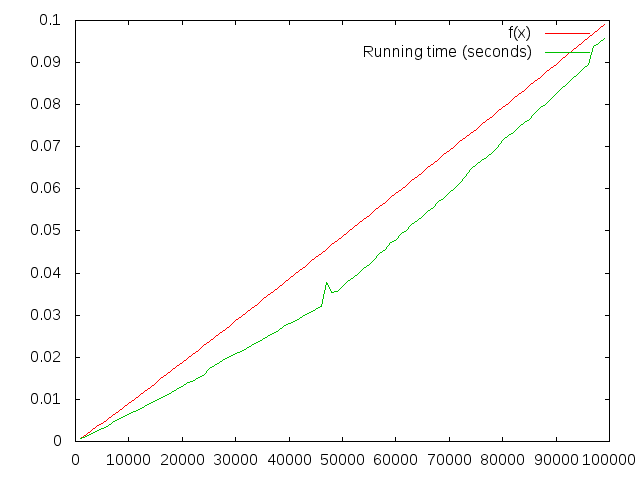
\includegraphics[scale=0.5]{erat3.png}
	\end{figure}
	
	It is evident from figure \ref{runtime1} that the function derived from the running time analysis bounds the experimental running time. So, we have a proven, efficient method for generating prime numbers up to some value.
	
	\section{Improvements and a New Sieve}
	
	Here we will begin discussing improvements to the sieve algorithm, and derive a different way to obtain prime numbers. The sieve of Sundaram operates on similar principles as the sieve of Eratosthenes, but has some differences that make it noteworthy when discussing prime generation.
	
	The sieve of Sundaram begins with a similar idea to the previous algorithm; we want to ``mark" or otherwise collect composite numbers, that are multiples of prime numbers. However, we can take advantage of an interesting result presented in lemma \ref{ijstuff} with regards to odd composite numbers.
	Once the algorithm has been presented, its asymptotic running time can be proved. We also demonstrate a plot of running time against output size, as we did with the sieve of Eratosthenes.
	
	\subsection{How to Find Odd Composites}
	
	Odd numbers can easily be written as $2k+1$ for some integer $k$. When we are trying to sieve primes, we would like to exclude those odd natural numbers that are composite; that is to say, those numbers that have a nontrivial factor. If we have some odd integer $a\geq3$, we can determine under what conditions $a$ is composite or prime.
	
	\begin{lem}\label{ijstuff}
		Let $a\geq3$ be an integer. Then $a$ can be written as $a = 2k+1$ where $k$ is of the form $k=i+j+2ij$, for nonnegative integers $i$ and $j$, if and only if $a$ is a composite number.
	\end{lem}
	\begin{proof}
		We can write $a$ as
		$$ 2k + 1 = 2(i+j+2ij) + 1 . $$
		Then we can simplify to obtain
		\begin{equation*}
		\begin{split}
		a &= 2(i+j+2ij) + 1 \\
		  &= 4ij + 2j + 2i + 1 \\
		  &= 2j(2i+1) + 2i + 1 \\
		  &= (2j+1)(2i+1)
		\end{split}
		\end{equation*}
		So $a$ is an odd composite number, since it has nontrivial odd factors $2j+1$ and $2i+1$.
	\end{proof}

	This result gives precisely the odd numbers where we can find primes. Now we can modify the sieve to cross out integers of the form $i+j+2ij$ up to $n$, and then obtain primes as those $2k+1$ for $3 \leq k \leq n$ that have not been crossed out.
	
	\subsection{The Sieve of Sundaram}
	
	This result was shown by an Indian mathematician, S. P. Sundaram in 1934 \cite[p.~158]{ogilvyanderson}. Unfortunately, little is known about him, besides his invention of this sieve. 
	
	Applying lemma \ref{ijstuff}, we can write a new algorithm.

	\begin{Algorithm}[H]\caption{Sieve of Sundaram}
        \begin{lstlisting}[language=Python]
        from math import ceil
        
        def Sundaram(n):
            interesting_nums = set()
            bound = int(ceil((n-2)/2))
            for i in range(1, bound):
                for j in range(i, int(ceil((n-i)/(1+2*i)))):
                    interesting_nums.add(2*i*j+i+j)
        
            return [2*a+1 for a in range(1,bound) if a not in interesting_nums]
        
        \end{lstlisting}
	\end{Algorithm}

	Again, we use the set structure because of its efficiency in membership checking. This time, we use nested loops for $i$ and $j$. The proof of correctness follows easily from lemma \ref{ijstuff}.
	
	\begin{thm}
		The algorithm \texttt{Sundaram} produces the prime numbers in the range $[3, n]$.
	\end{thm}
	\begin{proof}
		The final output contains only those integers between $3$ and $n$ which are not of the form $2ij+i+j$, as these have been culled into \texttt{interesting\_nums}. We know from lemma \ref{ijstuff} that for some $a=2k+1$, if $k$ is not of the form $2ij+i+j$, $a$ is prime. So, the final output contains all such $2k+1$ for $k$ not of the form $2ij+i+j$. The algorithm has total correctness as its loop bounds are finite.
	\end{proof}
	
	\begin{thm}
		The algorithm \texttt{Sundaram} has an asymptotic running time of $O(n^2)$.
	\end{thm}
	\begin{proof}
		Once again, we will count the number of set update operations performed. We have
		\begin{equation*}
		\begin{split}
		\sum_{i=1}^{\ceil*{\frac{n-2}{2}}} \sum_{j=i}^{\ceil*{\frac{n-i}{1+2i}}} 1 & = \sum_{i=1}^{\ceil*{\frac{n-2}{2}}} \ceil*{\frac{n-i}{1+2i}} - i + 1 \\
		& = \sum_{i=1}^{\ceil*{\frac{n-2}{2}}} \ceil*{\frac{n-i}{1+2i}} - \frac{1}{8}(n^2-2n) + \ceil*{\frac{n-2}{2}}
		\end{split}
		\end{equation*}
		If we ignore the first term, we can see that the remaining terms are on the order of $n^2$. The first term is a difficult summation to solve, so instead we will create an upper bound on the summand. Because the upper bound of the summation is linear in $n$, we expect a result of $O(n^2)$.
		\begin{equation*}
		\begin{split}
		\frac{n-i}{1+2i} < \frac{n-i}{2i} < \frac{n-i}{i} & = \frac{n}{i} - 1 < \frac{n}{i} < n
		\end{split}
		\end{equation*}
		If we use $n$ to replace $\ceil*{\frac{n-i}{1+2i}}$ in the above summation, we obtain
		$$\frac{1}{2}(n^2 - 2n)$$
		and so the resulting function of the runtime analysis is $O(n^2)$.
	\end{proof}
	
	Again, we can construct a time experiment to observe the running time in practice. The results are shown in figure \ref{runtime2}. On first glance, the plot appears linear, but upon careful consideration, quadratic curvature can be observed. Note also that the sieve of Sundaram appears slower than the sieve of Eratosthenes by a factor of about two on an output size of 100000.
	
	\begin{figure}\caption{Asymptotic Running Time of \texttt{Sundaram}}
		\label{runtime2}
		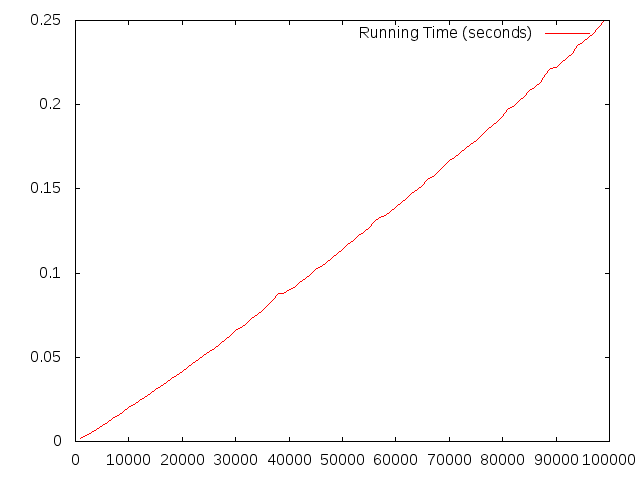
\includegraphics[scale=0.5]{sund2.png}
	\end{figure}
	
	\section{Comparison of the Two Sieves}
	
	This section will describe the two sieve algorithms we have seen and compare running time in theory and practice. We will elaborate on the details of each algorithm's shortcomings and strengths, with an interest in moving towards developing a more efficient sieve for large numbers.
	
	\subsection{Time Complexity and Practical Running Time}
	The first point to make is a comparison of the mathematically derived asymptotic running time for each sieve. While Sundaram is polynomial, Eratosthenes beats it by having a time complexity greater than linear but less than quadratic time. A comparison of theoretical asymptotic running times shows that Eratosthenes is a clear winner.
	
	Noting that practical considerations are also of importance, we can test the running time as a function of output size, running each algorithm several times and taking an average. The result of a side-by-side time trial gives the plot shown in figure \ref{runtimevs}. While Sundaram's sieve is slow with respect to Eratosthenes's sieve, it still beats trial division by a wide margin, shown in figure \ref{runtimetds}.
	
	\begin{figure}\caption{Comparison of Running Times of Both Sieves}
		\label{runtimevs}
		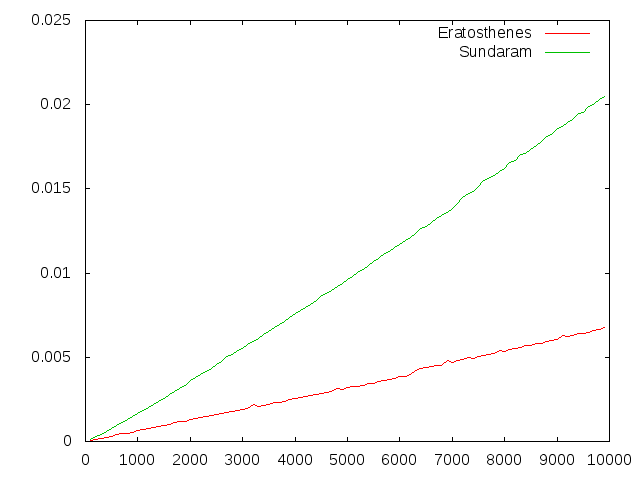
\includegraphics[scale=0.5]{both1.png}
	\end{figure}
	
	\begin{figure}\caption{Comparison of Running Times of Sundaram and Trial Division}
		\label{runtimetds}
		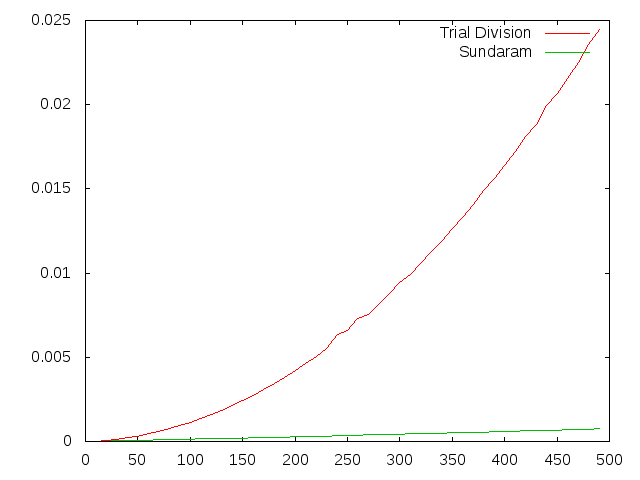
\includegraphics[scale=0.5]{sundiv.png}
	\end{figure}
	
	So, even when sieving smaller primes, Eratosthenes wins. Sundaram's algorithm makes clever use of lemma \ref{ijstuff}, but is still computationally inferior to Eratosthenes.
	
	\subsection{Strengths and Weaknesses}
	Intuitively, the sieve of Sundaram seemed like a potential contender against the sieve of Eratosthenes, but lost in terms of speed. The likely reason for this is the necessity to compute many numbers of the form $i+j+2ij$. The sieve of Eratosthenes has no such computation; it does not perform arithmetic when marking composite numbers, but merely iterates over multiples of primes, which is less computationally intense.
	
	That said, the sieve of Eratosthenes is simple, and we may intuitively believe there to be a more efficient solution. The sieve of Eratosthenes has asymptotic running time of $O(n \log \log n)$, which is sub-polynomial and therefore fast in practice. Both algorithms, however, are old. One may be inclined to ask whether there exists a contemporary sieve that operates in an even better time complexity than the sieve of Eratosthenes.

	\section{Reaching toward Linear Time: The Sieve of Atkin}
	
	We have seen two sieves that generate prime numbers up to some bound. In this section, we present the final sieve of our study, the sieve of Atkin. This algorithm again marks primes and composite numbers up to some limit, but the methods of marking here are vastly different. The theory that leads to the algorithm is considerably more involved than what was presented for the other sieves. Code for the algorithm is provided, and the asymptotic running time and correctness are shown.
	
	\subsection{Remainders and Modular Arithmetic}
	
	The process of sieving in Atkin's algorithm follows a very different set of rules from the sieves of Eratosthenes and Sundaram. We begin with a list having an entry for every positive integer. Each integer should be marked composite to begin with. Then, for every number $n$ in the sieve, compute $r = n \mod 60$. If $r \in \{1, 13, 17, 29, 37, 41, 49, 53\}$, we compute the number of solutions to $4x^2 + y^2 = n$, and negate the corresponding list entry for $n$ once for every solution we obtain. Similarly, if $r \in \{7, 19, 31, 43\}$ we compute solutions to $3x^2 = y^2 = n$. Finally, if $r \in \{11, 23, 47, 59\}$ we compute solutions to $3x^2 - y^2 = n$, $x>y$. If $r$ is not any of these, do nothing.
	
	Next, beginning with the lowest number in the sieve, we move to the next number marked prime, and include it in the output list of primes. Then, we square the prime and mark the multiples of the square as composite. We repeat these steps for numbers up to the square root of the upper limit. The output list then contains the primes up to the limit.
	
	The algorithm performs some computation before sieving, that involves looking for certain modulo 60 remainders. The full proofs regarding the quadratic forms are shown by Atkin and Bernstein \cite[p.~1028]{MR2031423}. Once these computations are finished, the sieve marks multiples of squares of primes, rather than multiples of the primes themselves. This leads to a better running time while iterating over the sieve.
	
	\begin{thm}
		The asymptotic time complexity of \texttt{Atkin} is $O(n^{3/2})$.
	\end{thm}
	\begin{proof}
		There are two separate iterations to consider: the \texttt{for} loop during preliminary computation, and the \texttt{for} loop during iteration over the sieve. For the former, we count modulo operations, and on the latter we count set discard operations. We can then write the running time as
		\begin{equation*}
		\begin{split}
		\sum_{x=1}^{\sqrt{n}} \sum_{y=1}^{\sqrt{n}} 4 + \sum_{i=5}^{\sqrt{n}} \sum_{j=i^2}^{n} 1 & = 4 \sum_{x=1}^{\sqrt{n}} \sqrt{n} + \sum_{i=5}^{\sqrt{n}} n - i^2 + 1 \\
		& = 4 \frac{\sqrt{n}(\sqrt{n}+1)}{2} + n\sqrt{n} - 4n - \frac{1}{6} (2n\sqrt{n} + 3n + \sqrt{n} - 180) + \sqrt{n} - 4 \\
		& = \frac{2}{3} n \sqrt{n} - \frac{5}{2} n + \frac{5}{2} \sqrt{n} + 26 \\
		& = O(n^{3/2})
		\end{split}
		\end{equation*}
		Note that an assumption was made in the fourth summation in the original expression, that $j$ starting at $i^2$ would iterate over every number up to $n$. This is not the case, as we iterate over multiples of $i^2$ up to $n$. This consideration would likely increase the complexity of the summation, but the outcome would still be a running time of $O(n^{3/2})$.
	\end{proof}
	
	\subsection{The Sieve in Practice}
	
	\begin{Algorithm}[H]\caption{Sieve of Atkin}
		\begin{lstlisting}[language=Python]
        import math
        
        def setflip(s, n):
            if n in s:
                s.remove(n)
            else:
                s.add(n)
        
        def Atkin(n):
            is_prime = set()
            for x in range(1, int(math.sqrt(n))+1):
                for y in range(1, int(math.sqrt(n))+1):
                    k = 4*x**2 + y**2
                    if k<=n and (k%12==1 or k%12==5):
                        setflip(is_prime, k)
                    k = 3*x**2+y**2
                    if k<= n and k%12==7:
                        setflip(is_prime, k)
                    k = 3*x**2 - y**2
                    if x>y and k<=n and k%12==11:
                        setflip(is_prime, k)
            for i in range(5, int(math.sqrt(n))):
                if i in is_prime:
                    for j in range(i**2, n+1, i**2):
                        is_prime.discard(j)
            return list(is_prime)
		\end{lstlisting}
	\end{Algorithm}
	
	The code is simplified by way of some simple observations. First, any number with a mod 60 remainder of 1, 13, 17, 29, 37, 41, 49, or 53 has a mod 12 remainder of 1 or 5. Any number with a mod 60 remainder of 7, 19, 31, or 43 has a mod 12 remainder of 1, and any number with a mod 60 remainder of 11, 23, 47, or 59 will have a remainder mod 12 of 11. By observing this, we trade computation of a few large modulo computations into a few more small ones.
	

	This running time analysis is performed on the code shown above. Indeed, Atkin showed a faster running time, and highly optimized versions of the sieve exist that run in linear time \cite[p.~1027]{MR2031423}. Still, we would like to take the results, and compare the practical running time to our very fast sieve of Eratosthenes.
	
	
	\section{Atkin versus Eratosthenes}
	
	In this section we begin by comparing the running time and complexity of the sieves of Atkin and Eratosthenes. We will again write a practical test to compare running time, but on a much larger scale than before. Both algorithms will be examined for shortcomings, and improvements discussed in the context of implementation optimizations.
	
	To begin, we revisit the theoretical running time of each algorithm in question. The sieve of Eratosthenes runs in $O(n \log \log n)$, whereas the sieve of Atkin runs in $O(n^{3/2})$. So, we should expect Eratosthenes to outperform Atkin, but the results will likely be close due to Atkin's quick sieve iteration. Again, we construct a test that times each algorithm on a number of output sizes. The results are plotted in figure \ref{runtimeeratkin}.
	
	\begin{figure}\caption{Comparison of Running Times of Eratosthenes and Atkin}
		\label{runtimeeratkin}
		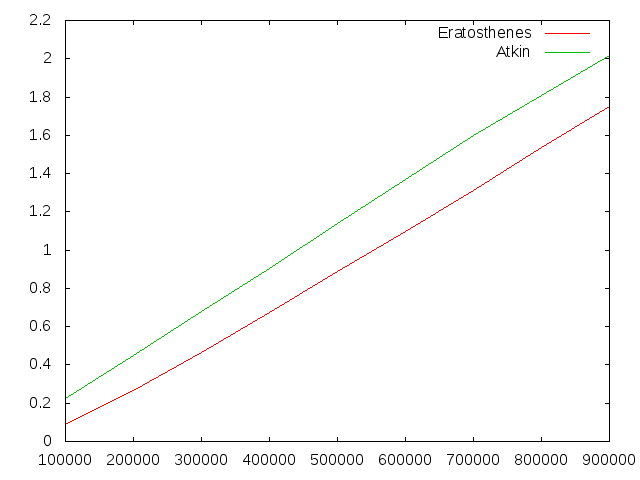
\includegraphics[scale=0.5]{eratkin1.png}
	\end{figure}

	This time, we have elected to run the sieves on very large output size, looking for primes up to one million, with the goal of escaping the dragging effect of the preliminary computations in the sieve of Atkin. Despite this, we still fail to see a point where Atkin overtakes Eratosthenes. The reasoning for this is likely twofold. First, the point where Atkin overtakes Eratosthenes may be a much larger number than one million, and the benefits of choosing Atkin over Eratosthenes may not be apparent until one attempts to generate primes of a much higher order of magnitude. Second, this simplified implementation of Atkin's sieve may not be enough to overtake Eratosthenes. Still, it is interesting to see the result; the sieves appear to be neck and neck.
	
	Both algorithms have potential for improvement in practice, when implementing the sieves. First, instead of using sets, a more efficient data structure could be used. While sets are good for membership checking, they take a lot of space, and could be replaced with something potentially more time efficient: bit arrays. One could initialize a bit array of length $n$, and let 0 and 1 represent prime and composite, or vice versa. Then, less space is used, and membership checking may be quicker as a result. Second, equipping sieves with wheel factorization aids in eliminating many more composite numbers more quickly.
	
	\section{Conclusion}
	
	After laying foundations in the theory of prime numbers, we discussed techniques and tricks that led to the intuitively simple sieve of Eratosthenes. After showing its time complexity and correctness, we worked toward a less trivial sieve due to Sundaram, and commented on its shortcomings when run against the sieve of Eratosthenes. Next, we showed that the contemporary sieve of Atkin was a potential contender against the sieve of Eratosthenes, and after elaborating on the algorithm, raced the two sieves. We found that despite large output size and the sieve of Atkin's preliminary work, Eratosthenes still won the race. Further improvements could be made to the algorithms present, were they to be implemented for general use. 
	
	Several further topics of interest are related to prime sieves. First, applications of prime generation to the RSA cryptosystem are of interest. Generally, a sieve-like method is used to filter out composite numbers from a range of large numbers, and primality tests are used to determine prime numbers from the range. Second, primality testing arises naturally when discussing RSA or prime number generation. Until 2004, primality testing was thought to be outside the reach of a polynomial time algorithm. Agrawal, Kayal, and Saxena demonstrated a polynomial time algorithm in a paper simply titled ``Primes is in P" \cite{MR2123939}. Despite this, probabilistic tests still tend to perform better than the AKS test.
	
	Future work may yet be done on prime sieves to improve an existing sieve's asymptotic running time. Alternatively, an entirely new sieve could be developed with a novel method of determining composite numbers. For the time being, however, the sieve of Eratosthenes and the sieve of Atkin are the standard tools in practice for generation of primes.
	

	\bibliographystyle{plain}
	\bibliography{termpaper2}


\end{document}